
\section{Introduction}
Modelling an object in 3D using software is a tedious and time consuming task. It is often done using very advanced and expensive software and becomes increasingly difficult as the complexity of the object is increased. If you're trying to model a physical object, a 3D scanner can be extremely useful. 
This will enable you to model an object with the scanning tool, and in a matter of minutes you have a complete digital 3D model. In many lines of work, this can speed things up tremendously, i.e. when doing research and development. 3D profiling can also be used for volume determination of an object.\\


There are multiple different starting points when designing and building a 3D scanner, but they're typically using either laser triangulation or structured light. There are even smartphones now, that can do simple 3D scans using LIDAR technology.
For our scanner, we will use a structured light source that will illuminate the object which is rotating on a stage, and a camera to capture images, see figure \ref{fig:setupintro} for a visualization of the test setup. 
\begin{figure}[h]
    \centering
    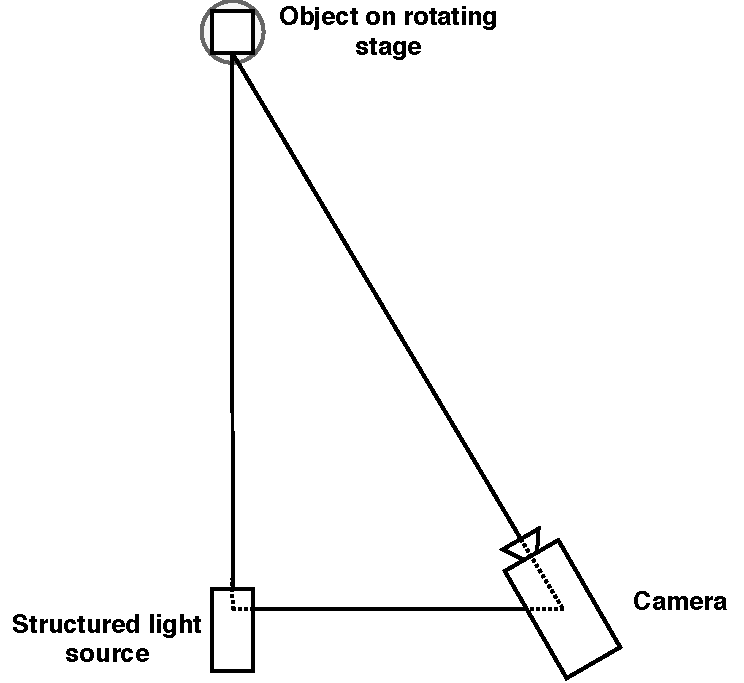
\includegraphics[width=0.5\textwidth]{figures/Introduction/setupIntroduction.pdf}
    \caption{Simple visualization of the test setup}
    \label{fig:setupintro}
\end{figure}

\newpage
\subsection{Objectives}
In this section, the objectives of the project are defined. These are milestone goals which are fundamental for the success of the project. The objectives are:
\begin{itemize}

    \item Derive the equations needed to gain depth information from structured light.
    \item Calibrate lens and camera to remove distortion and get intrinsic parameters of camera.
    \item Extract the structured light hitting the object.
    \item Track the movement of the structured light. 
    \item Combine above goals to recreate object in 3D.

\end{itemize}
\subsection{Constraints}
To reduce the scope of this project, a few constraints have to be considered:
\begin{itemize}
    \item Only one type of structured light will be explored.
    \item No stand-alone setup will be considered.
    \item Build-in implementations of different image analysing tool and filters will be used to evaluate performance of different methods, in order to reduce implementation time. 
\end{itemize}



% \begin{itemize}
%     \item The purpose of the project
%     \item Our approach  vs others (grid vs line, no laser), structured light in general
%     \item Scope
%     \item Problem formulation /Objectives 
%     \item Rough outline /setup with photos
%     \item Report overview
%     \item Table of contents 
% \end{itemize}






% \subsection{Objectives}
% \subsection{Constraints}
% \subsection{Outline of setup}
\subsection{Report overview}
\begin{itemize}
    \item \textbf{Chapter 2:} Introduction to camera models and derivation of the mathematical equations needed to estimate the object depth. Introduction of the overall setup for gathering data.
    \item \textbf{Chapter 3:} Calibration of camera and lens, both theory and implementation. 
    \item \textbf{Chapter 4:} Different methods for extracting structured light from images and tracking of movement.
    \item \textbf{Chapter 5:} Performance of proposed 3D reconstruction system.
    \item \textbf{Chapter 6:} Discussion of aspects which could have been done differently to improve performance and limit sources of errors
    \item \textbf{Chapter 7:} Conclusion
    \item \textbf{Chapter 8:} Future work 
    \item \textbf{Bibliography:} Bibliography with references used throughout the report
    \item \textbf{Appendix: A} Code for camera calibration
    \item \textbf{Appendix: B} Code for initializing depth reconstruction
    \item \textbf{Appendix: C} Code for 3D point cloud creation
    \item \textbf{Appendix: D} Other functions
\end{itemize}

% Define scope of project
% Define scope of camera calibration (only a tool)